\Chapter{Experimental Results}\label{sec:SIGNATURE}

In this chapter we present a method of determining the model that is closest to the ground thruth by defining a space to characterize models based on their predictive performance.  A real data set is a point in that space, and synthetic data sets associated with each model are also individual points.  The model's synthetic data set that is the closest to the real data set is deemed the ground truth.  Details of this framework is described later. We first review the basic concepts and the models used in this study.


\section{Model fit in a vector space framework}

The approach we propose to finding the model that best fits a data set is based on the assumption that the predictive performance of a given model will vary as a function of the data set's groud truth model, and that the relative performance between different data sets will be stable.

Let us explain this idea with the performance data in table~\ref{tab:vectorspace}, where the predictive accuracy of 6~well known skills models is reported against 6~synthetic data sets generated with the same models.  A seventh ``model'' named \textit{expected} and seventh data set named \textit{random} are added for comparison purpose.  The details of the different models and of the methodology to assess model performance are described later.  For now, let only focus on this table's data.

\newcolumntype{d}[1]{D{.}{.}{#1}} % not used

\begin{table}[ht]
\caption{Vector space of accuracy performances}\label{tab:vectorspace}
\centering
\begin{tabular}{lccccccc}
  \toprule
  \multicolumn{1}{c}{\multirow{2}{*}{\textbf{Model}}} & \multicolumn{7}{c}{\textbf{Synthetic data set}}\\
  \cline{2-8}
  & \multicolumn{1}{c}{{\textit{Random}}} & \multicolumn{1}{c}{{POKS}} & \multicolumn{1}{c}{{IRT}} & \multicolumn{1}{c}{{DINA}} & \multicolumn{1}{c}{{DINO}} & \multicolumn{1}{c}{{NMF.Conj}} & \multicolumn{1}{c}{{NMF.Comp}} \\ 
  \hline
  \textit{Expected} & \textbf{0.75} & 0.91 & 0.90 & 0.72 & 0.72 & 0.78 & 0.93 \\ 
  POKS & 0.75 & \textbf{0.94} & 0.94 & 0.81 & 0.81 & 0.90 & 0.94 \\ 
  IRT & 0.75 & 0.91 & \textbf{0.95} & 0.73 & 0.73 & 0.79 & 0.89 \\ 
  DINA & 0.75 & 0.77 & 0.81 & \textbf{1.00} & 0.65 & 0.98 & 0.89 \\ 
  DINO & 0.75 & 0.63 & 0.56 & 0.66 & \textbf{1.00} & 0.68 & 0.91 \\ 
  NMF.Conj & 0.75& 0.59 & 0.53 & 0.95 & 0.65 & \textbf{0.95} & 0.58 \\ 
  NMF.Comp & 0.75 & 0.76 & 0.79 & 0.59 & 0.93 & 0.70 & \textbf{0.98} \\ 
  \bottomrule
\end{tabular}
\end{table}


As we can expect, the diagonal (in bold face) always displays the best performance since it corresponds to the alignment of the model and the ground truth behind the data.  This confirms the intuition behind the usual strategy of assuming the best performer is the model behind the ground truth.  However, this is not always the case as we will see later.

The principle of the proposed approach is to use the whole column of performance as a vector to determine the closest model to the ground truth.  In that respect, if columns are considered as vectors in the space of dimensions created by model performances, we can use a similarity measure to determine the closest ground truth (or a distance measure if we were to consider the columns as a point in space).

The advantage of this approach is that it does not rely on a single performance value to determine the goodness of fit, but instead on a set of performances over different models.  The hypothesis is that this set of performances provides a more reliable measure of the goodness of fit of a set of models.  In turns, we assume that this measure is more likely to indicate which model will perform better in general, as opposed to which models performs the best in the case of the single data set at hand.  

The approach can be considered as a means to avoid a kind of local minimum, considering the best performer as a good indicator of the ground truth, but not a perfect one. Indeed, table\ref{tab:vectorspace} suggests that aligning the model with the ground truth does yield the best performance, but we will show examples later that there are exeptions and that the proposed approach is better able to avoid these exceptions that would lead to a wrong conclusion if we were to rely on the best performer approach.

\section{Skills Models}

The approach we introduce to assess model fit relies on the generation of synthetic data from different skills models.  We review the basics of each of these models.  We focus here on the assessment of static skills, where we assume the test data represents a snapshot in time, as opposed to models that allow the representation of skills that change in time, which is more typical of data from learning environments (see \citep{desmarais2012review}, for a review of both approaches).  However, the approach would generalize to dynamic data as well.

 For modeling static test data, Item Response Theory (IRT) is likely the most established model. It dates back to the 1960's and is still one of the prevailing approaches \citep{bakerKim2004}.  But, akin to the trend in data mining in general, many other models have been introduced in recent years.  Among them is the family of models that rely on slip and guess factors \citep{junker2001cognitive,Junker2000}, such as the DINA (Deterministic Input Noisy And-Gate), DINO (Deterministic Input Noisy Or-Gate), and other variants.  Other approaches are based on the Knowledge Space theory of Doignon and Falmagne \citep{Doignon1999}, which does not directly attempt to model underlying skills but instead rely on observable items only (\citep{desmarais:umuai:1995}; see also extentions that do include skills: \citep{heller2006competence}).  Finally, recent models based on matrix factorization have also emerged in the last decade \citep{Winters05,barnes2010novel,thai2011matrix,desmarais2012mapping}.  They factorize the student per item results matrix into the linear product of the so called Q-matrix (skills required per question item) and the skills mastery matrix.

There exists a large array of models to represent and assess student skills.  We focus here on the assessment of static skills, where we assume the test data represents a snapshot in time, as opposed to models that allow the representation of skills that change in time, which is more typical of data from learning environments (see \citep{desmarais2012review}, for a review of both approaches).

The skills assessment model we compare can be classified at a first level according to whether they model skills directly, and whether they are single or multiple skills.  Then, multi-skills model can be further broken down based on whether they have guess and slip parameters, and whether the skills are considered disjunctive or conjunctive.  Figure~\ref{AssessMethods} shows this hierarchy of models.

\begin{figure}[ht]
\centering
   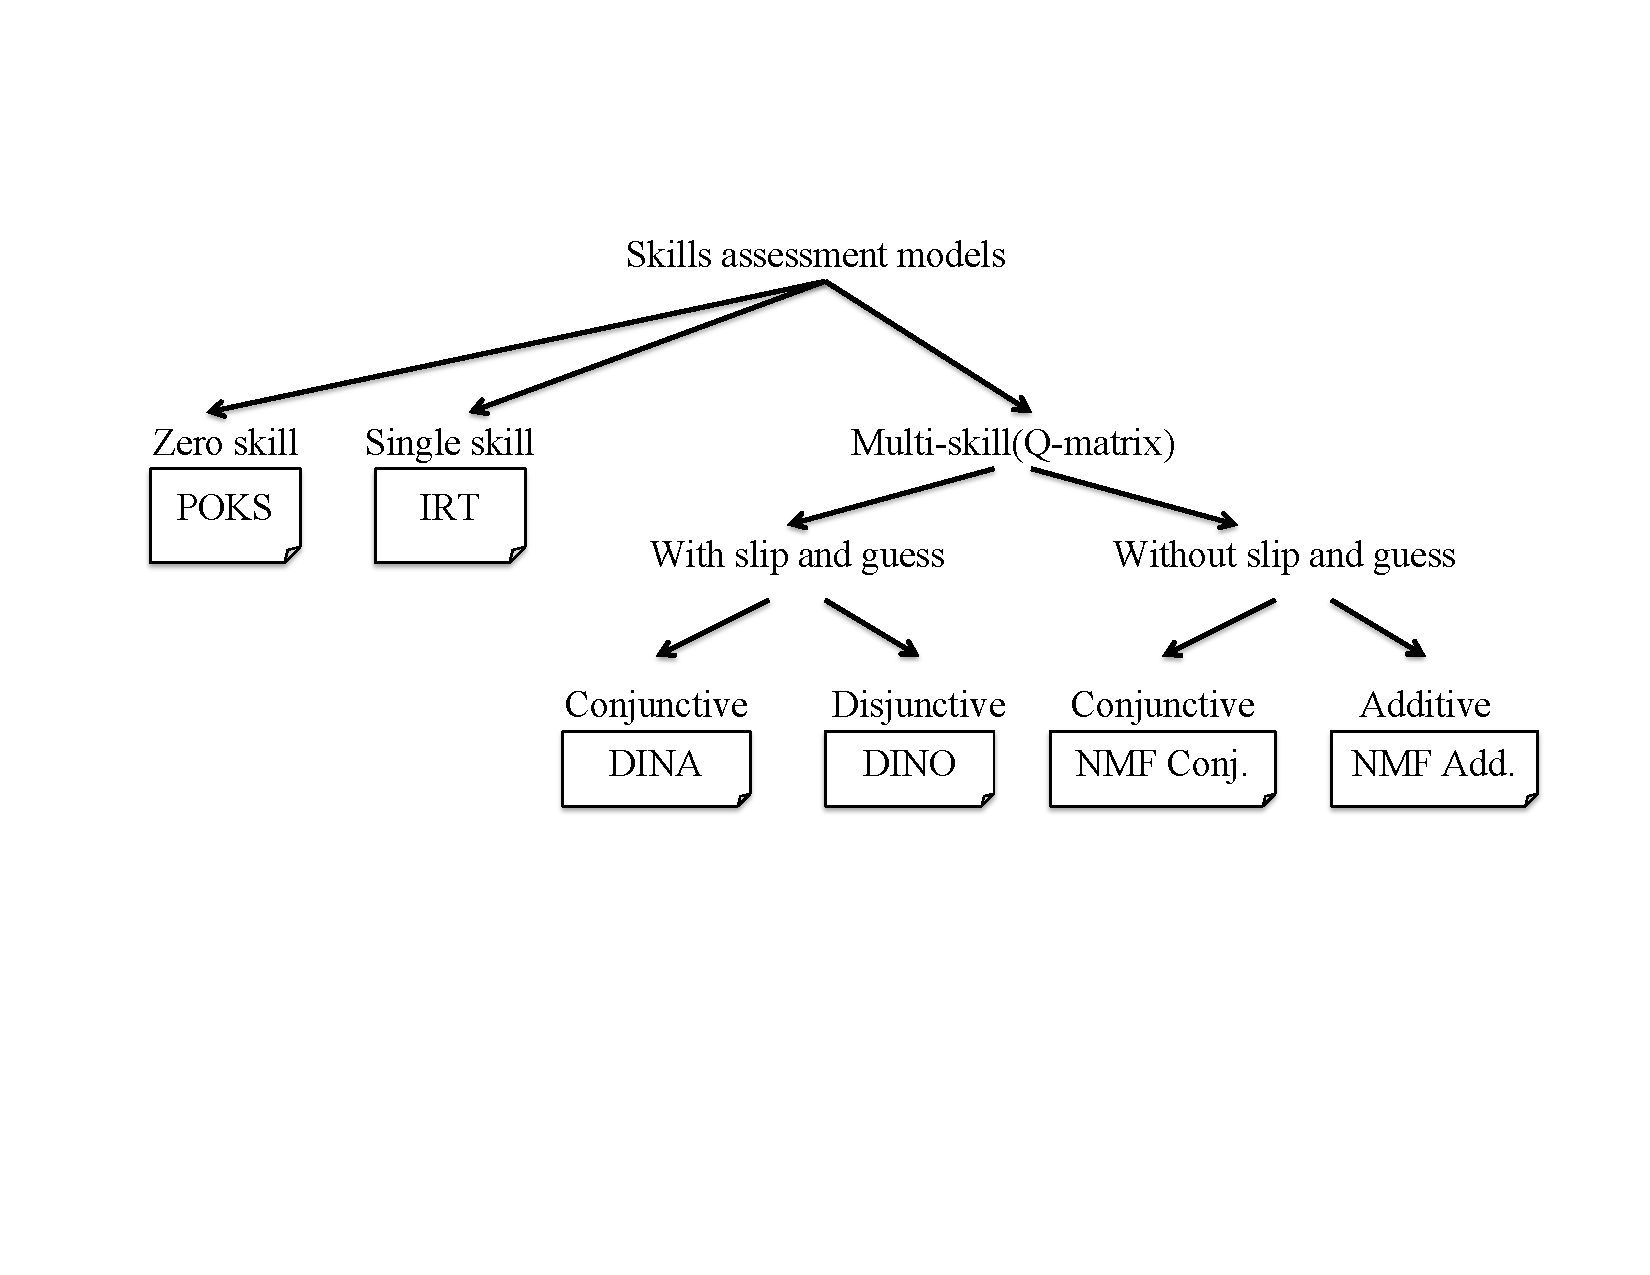
\includegraphics[trim=0.5cm 7cm 0.5cm 3cm,scale =0.5] {SkillsAssessments.pdf}
\caption{Skills assessment methods}
\label{AssessMethods}
\end{figure}

The POKS model avoids the specification of skills alltogether by modeling the order in which items or tasks are learned.  Skills can be be modeled in a second phase once these items are mapped to given skills.  IRT is a well established family of models that rely on a single skill to model student performance data.  Finally the multi-skill family of models rely on a mapping of item to skills, called a Q-matrix.  The DINA model incorporates the guess and slip parameters and considers the all skills specified in a Q-matrix as required in order to succeed an item, whereas the DINO model requires any skills to be sufficient.  The NMF conjunctive and NMF additive models are the counterpart of DINA and DINO, but they do not incorporate the guess and slip parameters, and the NMF additive model is closer to a continuum between conjunction and disjunction, as every skill mastered is considered to increase the chances of success as opposed to strict a disjunction for which any single skill is sufficient.






\section{Methodology}

In a first experiment, we focus on showing the performance of all models over synthetic and real data sets.  It provides an overview of the relative performance of each model across the different synthetic data sets and across real data as well. 

In a second experiment, we move focus to the central problem of this paper: classifying data sets in the performance vector space.  To validate the approach, we need to rely solely on synthetic data for which we know the underlying ground truth model.  A matrix such as the one in figure~\ref{AssessMethods} is created with data sets generated from the different models, and each model performance is measured through a cross validation process.  This matrix allows us to classify a data set of unknown ground truth according to a nearest neighbour approach.  

%%%%%%%%%%%%%%%%%%%%%%%%%%%%%%%%%%%%%%%%%%%%%%%%%%%%%%%%%%%%%%%%%%%%%%%%%%%%%
\section{Experiment 1: Performance comparison}

The performance of each model is assessed on the basis of 10-folds cross-validation.  The training set is used to estimate model parameters that are later used in for the test set. For each test set, a model is fed with a set of item outcomes of a student, called the observed set, and the remaining items are the predicted, or inferred ones. The breakdown of the data for cross-validation is illustrated in figure~\ref{figMethod}. We fixed the number of observed items for each run on each data set. The minimum number of observed items is 9 and the maximum number is one item less than total number of items. 

\begin{figure}
\centering
{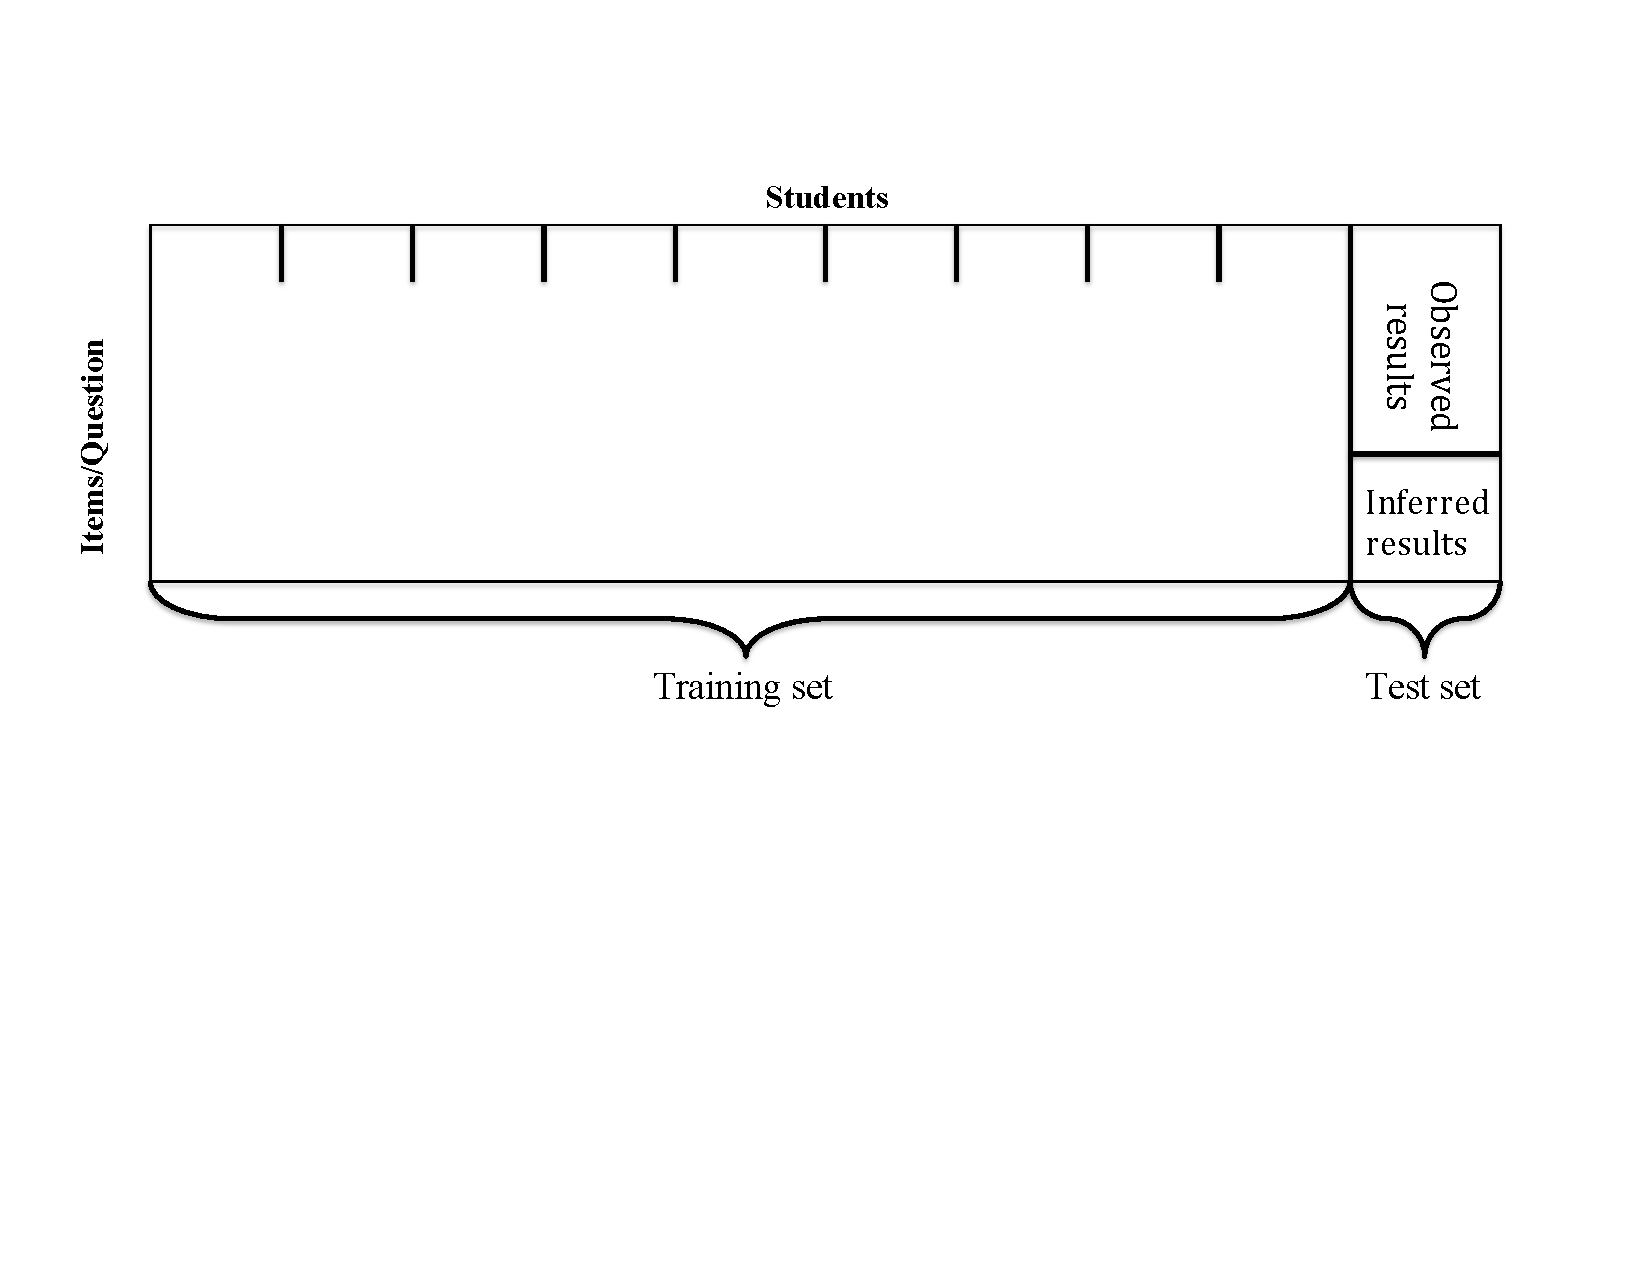
\includegraphics[trim=2cm 9cm 2.4cm 2.4cm,clip=true,width=.6\textwidth]{Images/Methodology.pdf}}
\caption{Data breakdown of cross validation process}
\label{figMethod}
\end{figure}

For each dataset there exists a training set that contains 9 folds and a test set that which represents a single fold. A list of required parameters are presented in table~\ref{fig:param}. Samples are assigned randomly to each fold and this setting is the same across all predictive models for each run. Since all items are presented in the training set, then we can estimate the parameters that are related to items. 

\begin{table}
  \centering

  \begin{tabular}{>{\raggedright}p{.02\textwidth}>{\raggedright}p{.3\textwidth}>{\raggedright}p{.15\textwidth}>{\raggedright}p{.4\textwidth}}
    \toprule
    & \multicolumn{1}{c}{\textbf{Parameter}} & \multicolumn{1}{c}{\textbf{Typical values}} & \multicolumn{1}{c}{\textbf{Models affected}} \tabularnewline
    \toprule
    \multicolumn{3}{l}{\textbf{Data specific parameters}}\tabularnewline
    \cline{2-4}
    & Number of skills & \numrange{3}{9} & Multiple skills models:\newline DINA, DINO, NMF Conj./Add. \tabularnewline
    \cline{2-4}
    & Number of items & \numrange{10}{50} &   \tabularnewline
    \cline{2-3}
    & Number of students & \numrange{100}{1500} & \tabularnewline
    \cline{2-3}
    & Test success rate & \numrange{0.25}{0.85}   &\tabularnewline
    \cline{2-3}
    & Student score variance & \numrange{0.03}{0.20} & \tabularnewline
    \cline{2-3}
    & Item score variance & \numrange{0.03}{0.20} & \multirow{-5}{*}{All models} \tabularnewline
    \cline{2-4}
    & Item discrimination & \numrange{0.5}{3} & \tabularnewline
    \cline{2-3}
    & Item difficulty & \numrange{-3}{3} & \tabularnewline
    \cline{2-3}
    & Student ability & \numrange{-4}{4} & \multirow{-3}{*}{IRT} \tabularnewline
    \hline
    \multicolumn{3}{l}{\textbf{Simulation parameters}}\tabularnewline
    \cline{2-4}
    & Number of observed items &  9 to Number of items -1 & \tabularnewline
    \cline{2-3}
    & Training set size & 90\% of $[100-1500]$ &  \multirow{-2}{*}{All models}\tabularnewline
    \hline
    \multicolumn{3}{l}{\textbf{Model specific parameters}}\tabularnewline
    \cline{2-4}
    & Guess and slip & $[0.0-0.2]$ & DINO and DINA\tabularnewline
    \cline{2-4}
    & Binomial and interaction tests & $\alpha_1=0.85\newline \alpha_2=0.10$ & POKS\tabularnewline
    \bottomrule
  \end{tabular}
  \caption{Parameters of the simulation framework}
  \label{fig:param}
\end{table}


\newcommand{\tabitem}{~~\llap{\textbullet}~~}
\newcommand\VRule[1][\arrayrulewidth]{\vrule width #1}



\begin{table}
  \centering

\begin{tabular}{c|c|l!{\VRule[1.5pt]}l|l!{\VRule[1.5pt]}l|}
\multicolumn{3}{c}{}&\multicolumn{3}{c}{Parameters estimated from}\tabularnewline
\cline{4-6}
\multicolumn{3}{c!{\VRule[1.5pt]}}{Skills Model}&\multicolumn{2}{c!{\VRule[1.5pt]}}{Training set}&Observed items\tabularnewline
\cmidrule[1.5pt]{2-6}
&&NMF Conj. & & &  \tabularnewline
\cline{3-3}
&&NMF Add.&&& \tabularnewline
\cline{3-4}
&&DINA& \tabitem Slip & &\tabularnewline
\cline{3-3} 
&\multirow{-4}{*}{\begin{sideways} \scriptsize Multiple\end{sideways}}&DINO& \tabitem Guess&\multirow{-4}{*}{ \tabitem  Q-matrix }&\multirow{-4}{*}{  \parbox[t]{3cm}{ \tabitem Students skills  \\ mastery matrix}} \tabularnewline
\cmidrule[1.5pt]{2-6}
&&&\multicolumn{2}{l!{\VRule[1.5pt]}}{\tabitem Item difficulty  } &  \tabularnewline
&&\multirow{-2}{*}{ IRT}&\multicolumn{2}{l!{\VRule[1.5pt]}}{\tabitem Item discrimination}  &\multirow{-2}{*}{\tabitem Student Ability} \tabularnewline
\cline{3-6}
&\multirow{-3}{*}{\begin{sideways} \scriptsize Single \end{sideways}}&Expected&\multicolumn{2}{l!{\VRule[1.5pt]}}{\tabitem Item Odds}  &\tabitem Student Odds \tabularnewline
\cmidrule[1.5pt]{2-6}
&&&\multicolumn{2}{l!{\VRule[1.5pt]}}{\tabitem Initial Odds } & \tabularnewline
&&&\multicolumn{2}{l!{\VRule[1.5pt]}}{ \tabitem Odds ratio } & \tabularnewline
\multirow{-9}{*}{\begin{sideways} \scriptsize Contributed skills \end{sideways}}&\multirow{-3}{*}{\begin{sideways} \scriptsize Zero\end{sideways}}&\multirow{-3}{*}{ POKS }&\multicolumn{2}{l!{\VRule[1.5pt]}}{\tabitem PO structure}&\multirow{-3}{*}{ }\tabularnewline
\cmidrule[1.5pt]{2-6}
\end{tabular}
  \caption{Parameters of the predictive performance framework}
  \label{fig:param-Predictive-Performance}
\end{table}


For other parameters that are related to students we need to divide the test set into an observed and inferred set. From the observed set we can get to the parameters that are related to students. A list of required parameters for assessing the model performance in table~\ref{fig:param-Predictive-Performance}.

Once all the required parameters are presented we can make a prediction for the inferred cells of the result matrix. Note that the selected observed and inferred items are the same across all the models for each run to make a better comparison for their prediction. A probability of mastery is obtained and rounded, resulting in a 0/1 error loss function.  We report the mean accuracy as the performance measure.  The R package \texttt{ltm} is used for parameter and skills estimation for IRT model and the R package \texttt{CDM} and \texttt{NMF} for Deterministic noisy and NMF models. A comparison between the predicted results and the real values can result in a performance accuracy. 


%%%%%%%%%%%%%%%%%%%%%%%%%%%%%%%%%%%%%%%%%%%%%%%%%%%%%%%%%%%%%%%%%%%%%%%%%%%%%
\subsection{Data sets}

The performance of the models is assessed over a total of 14~data sets, 7~of which are synthetic, and 7~are real data.  They are listed in table~\ref{tabl1}, along with the number of skills of their Q-matrix, their number of items, the number of the student respondents, and the average score.  Table~\ref{tabl1} also reports the Q-matrix used.  As can be seen, some synthetic data sets share their Q-matrix with real data sets.  This sharing allows greater similarity between the synthetic data and a real data counterpart that shares a Q-matrix.  Other parameters used to create the synthetic data sets were also obtained from real data sets with the same intent of allowing better comparison.  

Of the 7~real data sets, only three are independent.  The other~4 are variations of a well known data set in fraction algebra from Tatsuoka's work \citep{tatsuoka1984analysis}.  They consists in subsets of questions and variations of the Q-matrix.  These variants allows us to explore the effect of different models (Q-matrices) over the same data source.

The Vomlel data was obtained from \citep{vomlel:2004} and is also on the topic of fraction algebra.  The Q-matrix for this data is derived from the Bayesian Network defined over the 20~item test by experts.

The ECPE data (Examination for the Certificate of Proficiency in English) is an English as a foreign language examination. It is recognized in several countries as a test of advanced proficiency in English and used by a number of universities.

These real data sets were obtained from different sources and are freely available from the CDM \citep{Robitzsch2012} and NPCD ({\url{http://cran.r-project.org/web/packages/NPCD/}}) R packages. The Q-matrices of the real data sets were made by experts.


\newcounter{i}\setcounter{i}{1}
\newlength{\mdnum}
\setlength{\mdnum}{\widthof{10}}
\newlength{\mdnumtwo}
\setlength{\mdnumtwo}{\widthof{$\mathbf{Q}_{01}$}}
\newcommand{\mdcount}[2]{\parbox{#1}{\hfill\arabic{i}}.\ #2\addtocounter{i}{1}}
\begin{table}
\centering
\footnotesize
%\begin{tabular}{|l|c|c|r|r|l|}
\begin{tabular}{|l|c|c|r|r|l|}
\hline

%\rowcolor{\color[rgb]{.8,.8,.8}}
\multirow{2}{*}{Data set} & \multicolumn{3}{c|}{Number of} & {\parbox{6ex}{\center Mean\\Score}} & \multirow{2}{*}{Q-matrix}\tabularnewline
\cline{2-4} 
%\rowcolor{\color[rgb]{.8,.8,.8}}
 & Skills & Items & Students &  & \tabularnewline
\hline
\hline
%\rowcolor{\color[rgb]{.9,.9,.9}}
\multicolumn{6}{|c|}{\textit{Synthetic}}\\
\hline
\hline
\mdcount{\mdnum}{Random} & 7 & 30 & 700 &0.75& $\mathbf{Q}_{01}$\tabularnewline
\hline
\mdcount{\mdnum}{POKS} & 7 & 20 & 500 &0.50 & $\mathbf{Q}_{02}$\tabularnewline
\hline
\mdcount{\mdnum}{IRT-2PL} & 5 & 20 & 600 &0.50& $\mathbf{Q}_{03}$\tabularnewline
\hline
\mdcount{\mdnum}{DINA} & 7 & 28 & 500 &0.31& $\mathbf{Q}_5$\tabularnewline
\hline
\mdcount{\mdnum}{DINO} & 7 & 28 & 500 &0.69& $\mathbf{Q}_6$\tabularnewline
\hline
\multicolumn{6}{|l|}{Linear (Matrix factorization)}\\
\hline
\mdcount{\mdnum}{~~~Conj.} & 8 & 20 & 500 &0.24& $\mathbf{Q}_1$\tabularnewline
\hline
\mdcount{\mdnum}{~~~Comp.} & 8 & 20 & 500 &0.57& $\mathbf{Q}_1$ \tabularnewline
\hline
\hline
%\rowcolor{\color[rgb]{.9,.9,.9}}
\multicolumn{6}{|c|}{\textit{Real}}\\
\hline
\hline
\mdcount{\mdnum}{Fraction} & 8 & 20 & 536 &0.53& $\mathbf{Q}_1$\tabularnewline
\hline
\mdcount{\mdnum}{Vomlel} & 6 & 20 & 149 &0.61& $\mathbf{Q}_4$\tabularnewline
\hline
\mdcount{\mdnum}{ECPE} & 3 & 28 & 2922 &0.71& $\mathbf{Q}_3$\tabularnewline
\hline
\multicolumn{6}{|l|}{Fraction subsets and variants of $\mathbf{Q}_{1}$}\\
\hline
\mdcount{\mdnum}{~~~1} & 5 & 15 & 536 &0.53& $\mathbf{Q}_{10}$\tabularnewline
\hline
\mdcount{\mdnum}{~~~2/1} & 3 & 11 & 536 &0.51& $\mathbf{Q}_{11}$\tabularnewline
\hline
\mdcount{\mdnum}{~~~2/2} & 5 & 11 & 536 &0.51& $\mathbf{Q}_{12}$\tabularnewline
\hline
\mdcount{\mdnum}{~~~2/3} & 3 & 11 & 536 &0.51& $\mathbf{Q}_{13}$\tabularnewline
\hline
\hline
\end{tabular}
\caption{Datasets}
\label{tabl1}
\end{table}


The synthetic data sets are generated from each skills assessment model, with an effort to fit the parameters as closely as possible to a real data counterpart that shares the same Q-matrix.  

For POKS, the structure was obtained from the Fraction data set and the conditional probabilities were generated stochastically, but in accordance with the semantic constraints of these structures and to obtain an average success rate of 0.5.

For IRT, the student ability distributions was obtained from the Fraction data set, and the item difficulty was set to reasonable values: averaging to 1 and following a Poisson distribution that kept most values between 0.5 and 2 (done by generating random numbers from a Poisson distribution with lambda parameter set to 10 and dividing by 10). 

The matrix factorization synthetic data sets of DINO and DINA were generated by taking a Q-matrix of 7~skills that contains all possible combinations of 1 and 2~skills, which gives a total of 28~combinations and therefore the same number of items.  Random binary skills matrix (which corresponds to matrix~$\mathbf{S}$ in equation~(\ref{eq:1}) were generated and the same process was used for both the DINO and DINA data sets.  Item outcome is then generated according to equation~(\ref{DinoEQ}) with a slip and guess factor of 0.1.

A similar process was followed to generate the Q-matrices and the skills matrices~$\mathbf{S}$ of the linear matrix factorization data sets, except that item outcome follows equation~(\ref{eq:1}) and is discretized.

%% MD: Investigate differences in correlations between items across real vs. synthetic data

Note that the first 4~models do not rely on any Q-matrix for the data generation process, but the DINO/DINA and matrix factorization assessment models still require one.  To define these Q-matrices (denoted~$\mathbf{Q}_{0x}$ in table~\ref{tabl1}, a wrapper method was used to first determine the number of skills according to \citep{Beheshti2012Numbers}, then a Q-matrix was derived with the deterministic ALS algorithm as described in section~\ref{ALS-Def}, starting with an initial random Q-matrix.
%% MD: Behzad, is this right?


%%%%%%%%%%%%%%%%%%%%%%%%%%%%%%%%%%%%%%%%%%%%%%%%%%%%%%%%%%%%%%%%%%%%%%%%%%%%%
\subsection{Predictive performance results} \label{secSyn}

This section shows the result of predictive performance of the seven models over the 14~datasets described in table\ref{tabl1}. 

\begin{figure}
\centering
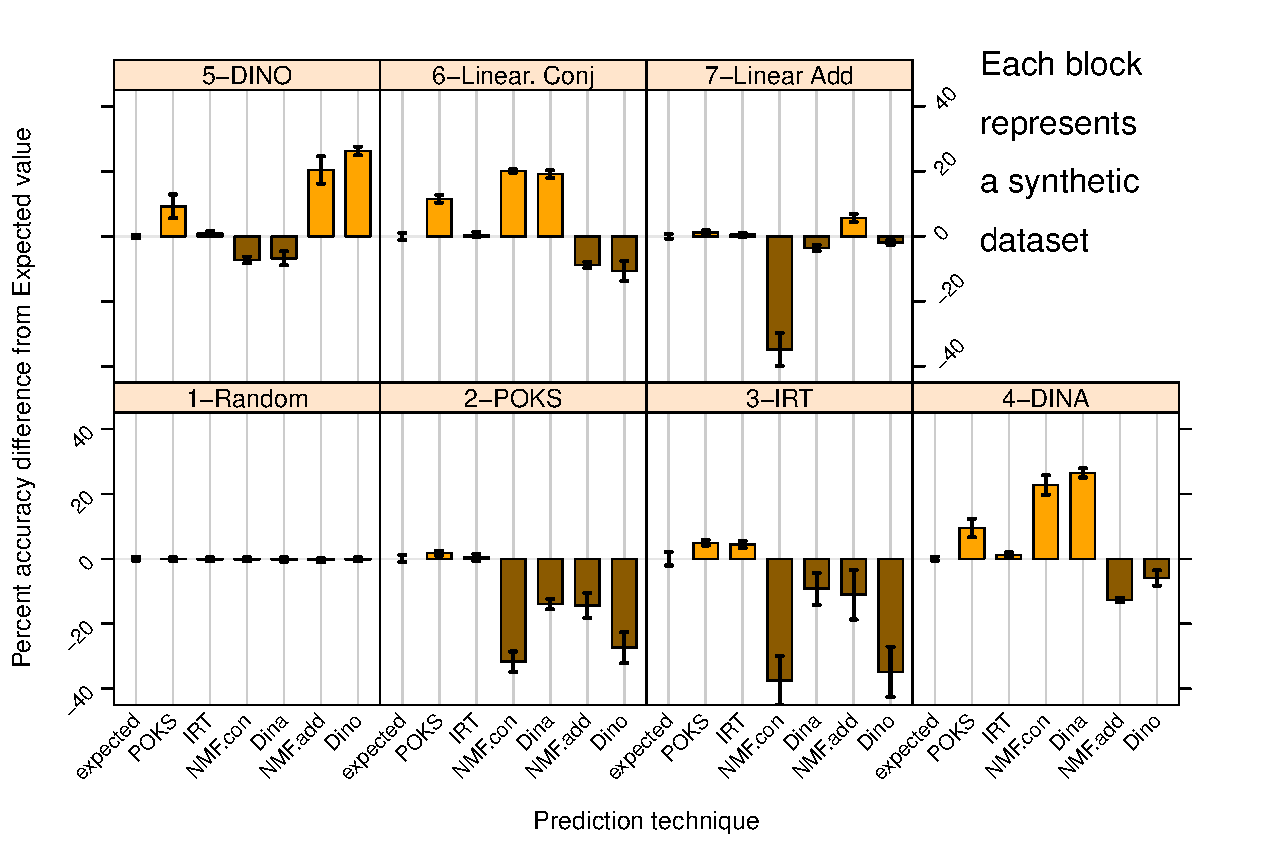
\includegraphics[clip=true,width=.9\textwidth]{Syn.pdf}
\caption{Item outcome prediction accuracy results of {\textbf{synthetic data sets}}}
\label{fig1}

{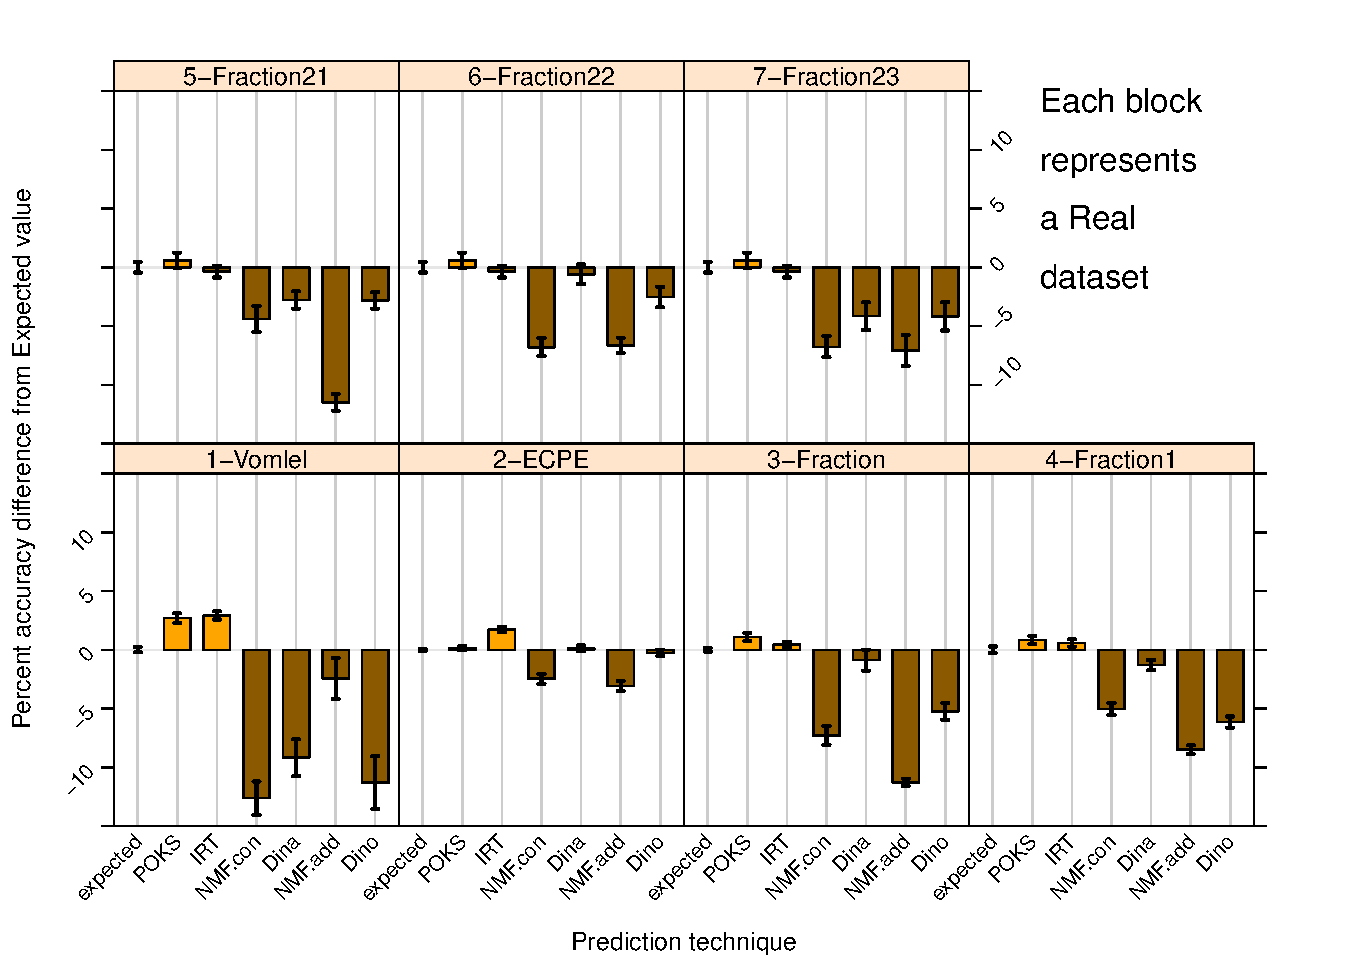
\includegraphics[clip=true,width=.9\textwidth]{Real.pdf}}
\caption{Item outcome prediction accuracy results of {\textbf{real data sets}}}
\label{fig2}
\end{figure}
%% We should eventually change the scale to logit so that the differences are more pronounced at the extremes
%% (or maybe just rescale from min-max for each data set)

Figures~\ref{fig1} and~\ref{fig2} show the performance of each model over the synthetic and real data sets.  The performance is the difference in accuracy of each model from the expected value, which serves as a baseline. Note that the y-scale of the synthetic data is double the one of the real data sets, and therefore the differences in performance for the synthetic datasets are much wider.  An error bar of 1~standard deviation is reported, computed over 10 simulation runs that each run considers four different number of observation that varies between 9 to an item less than maximum number of items, provides an idea of the variability of the results. A dataset of random data is also reported for a~$0.75$ average success rate.

As expected, when the generative model behind the synthetic data set is the same as the skills assessment technique, the corresponding technique's performance is the best, or close to the best.  And this performance is also always above the expected value performance, except for the random data set where not model can do any different than the expected value, which is what we would expect.

For the synthetic data sets, three models reach performances that are much higher than the baseline, in the range of $20-30$\% (DINO, Linear Conjunctive, and DINA), whereas for the three other models the gain is closer to 5\% (Linear additive, POKS, and IRT).

An important observation is that the pattern of relative differences of performances across techniques varies considerably and is unique to each data set: no two data sets have the same pattern of relative performance across models.  The capacity of recognizing a data set's true model relies on this uniqueness characteristic.

For the real data sets, the relative performance among the techniques shows smaller discrepancies and is closer to the baseline. Although the best performers are still significantly better than the expected values for the majority of the data sets, it is surprising to see that a majority of models do worst than the baseline for a majority of data sets. \remove{It does not seem always significant.}

The results from the subsets of the Fraction data show that the pattern of the Fraction performance data set repeats over Fraction-1, Fraction-2/1 and Fraction-2/2, in spite of the different number of skills and different subsets of questions.  However, it differs substantially from Fraction-2/3 for the NMF conjunctive performance which reaches that of the NMF additive one and also DINA reaches DINO. This is readily explained explained by the fact that the Q-matrix of this data set has the property of assigning a single skill to each item, in which case the two matrix factorization techniques become equivalent.  But aside from the Fraction-2/3 case, this similarity among Fraction data set and its derivative suggests that in spite of the model differences (different Q-matrices and item subsets), the performance ``signature'' remains constant across these data sets.

Finally, we note that none of the real data sets show the large the discrepancies found in the synthetic data sets models. One exception is the linear additive synthetic data set which displays smaller variance across models and which ``signature'' resembles the Vomlel data, although the performance difference with the majority class is substantially higher for the synthetic data than the Vomlel data, suggesting that the real data is yet not a perfect fit to this model.
%% MD: we need to test this with the same Q-matrices.

%\begin{figure}
%  \centering

%    \includegraphics[scale=0.6]{Images/numberofObs.pdf}
%     \caption{Synthetic datasets with different number of observation}
%\label{figSampleSize}
%\end{figure}

\section{Experiment 2: Sensitivity of the Model performance over data generation parameters}
\label{Sensitive}

In this experiment we want to examine the effect of data generation parameters on the stability of the model performance vector in the performance space. In this section we run the same experiment but with different parameters such as average success rate, sample size, number of latent skills, number of items, student and item score variance. These factors can can answer the question whether the patterns hold across different conditions. Table \ref{fig:param} shows different conditions of the parameters.

Just like the previous experiment, we assessed these results on the basis of 10-folds cross-validation. The same as before, we fixed the number of ``observed items'' for each run on each data set that varies between 9 to one item less than total number of items.

We generated the synthetic datasets with different sample size which varies from 100 students upto 1500 students. Figure~\ref{figSampleSize} shows the result of this change. Running all these techniques on the synthetic datasets did not change any pattern except for IRT generated dataset that slightly changed the pattern for small sample size. On the other cases the one with the highest predictive performance was the same as model behind the generated data. Also changing the sample size downto less than 100 students will change the pattern as well; because the training set of the model could not be Learned properly.


\begin{figure}
  \centering

    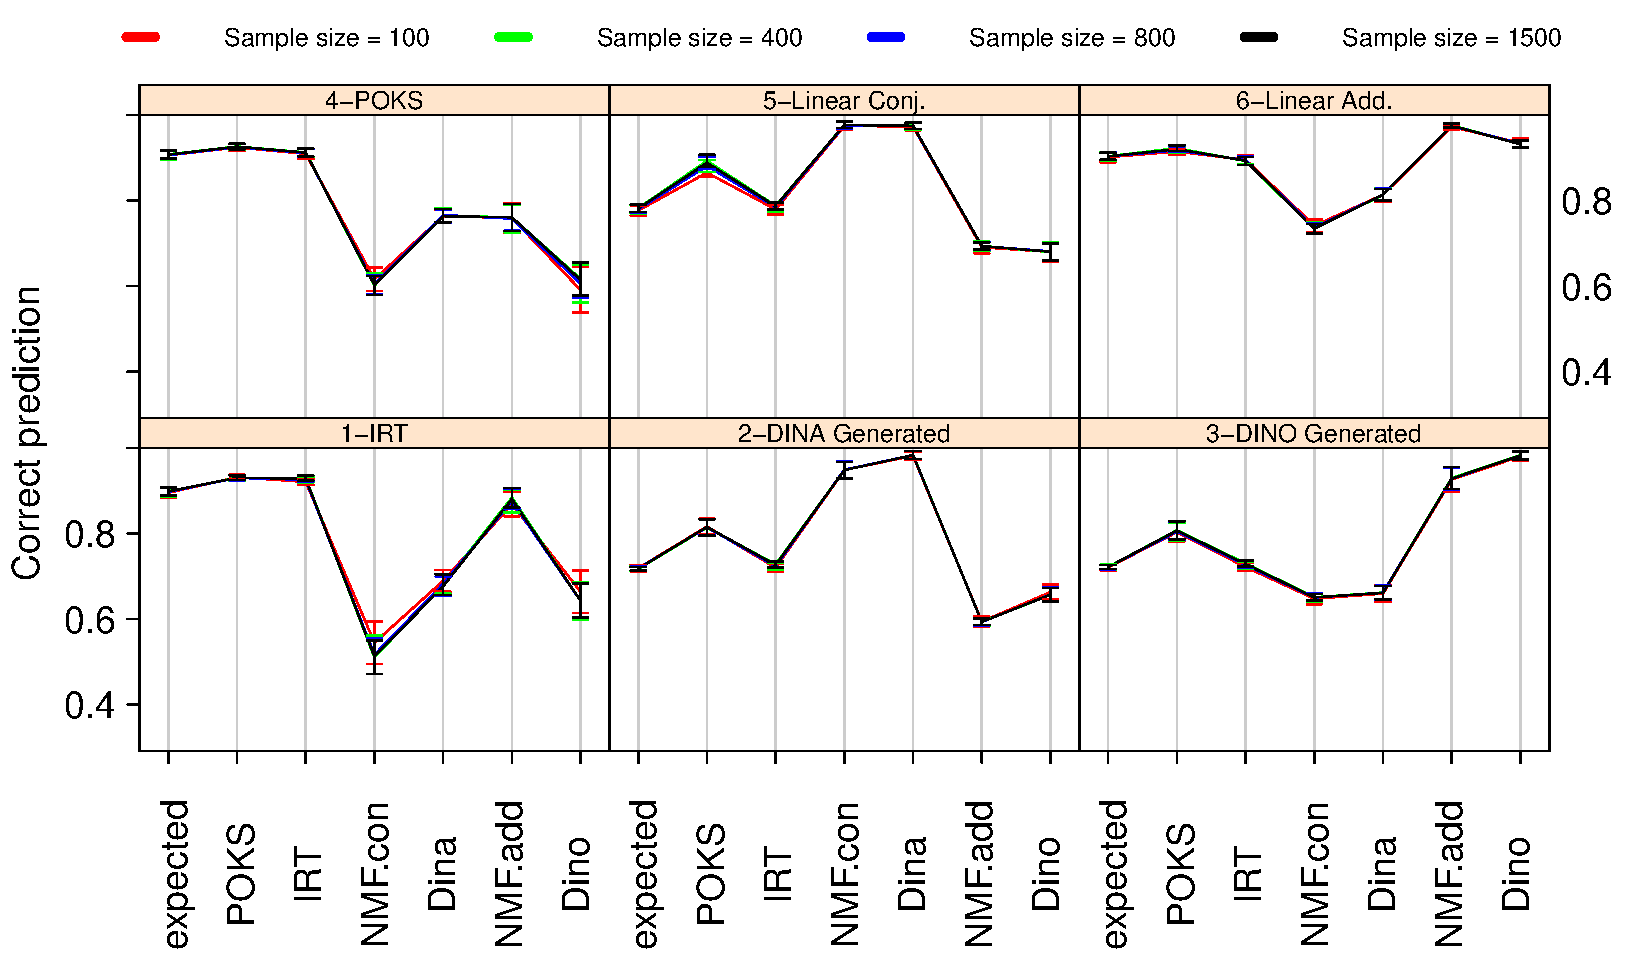
\includegraphics[scale=0.58]{SampleSize.pdf}
     \caption{Variation of \textbf{Sample Size} Over synthetic data sets}
\label{figSampleSize}
\end{figure}

The other parameter is the number of Items in generation of the synthetic dataset. This time we fixed all the other parameter but the Items size which varies between 10 to 50 items. Figure~\ref{figNumberofItems} shows how signature has been changed for different models. The results on the synthetic datasets shows that in some cases the pattern stays the same but it shifts down on the chart once we decrease the number of items. Still we can see that the highest performance is the same model behind the generated dataset. This highlights the role of this variable in predicting the signature and also means that the highest performance should not necessary be close to 100\%.

\begin{figure}
  \centering
    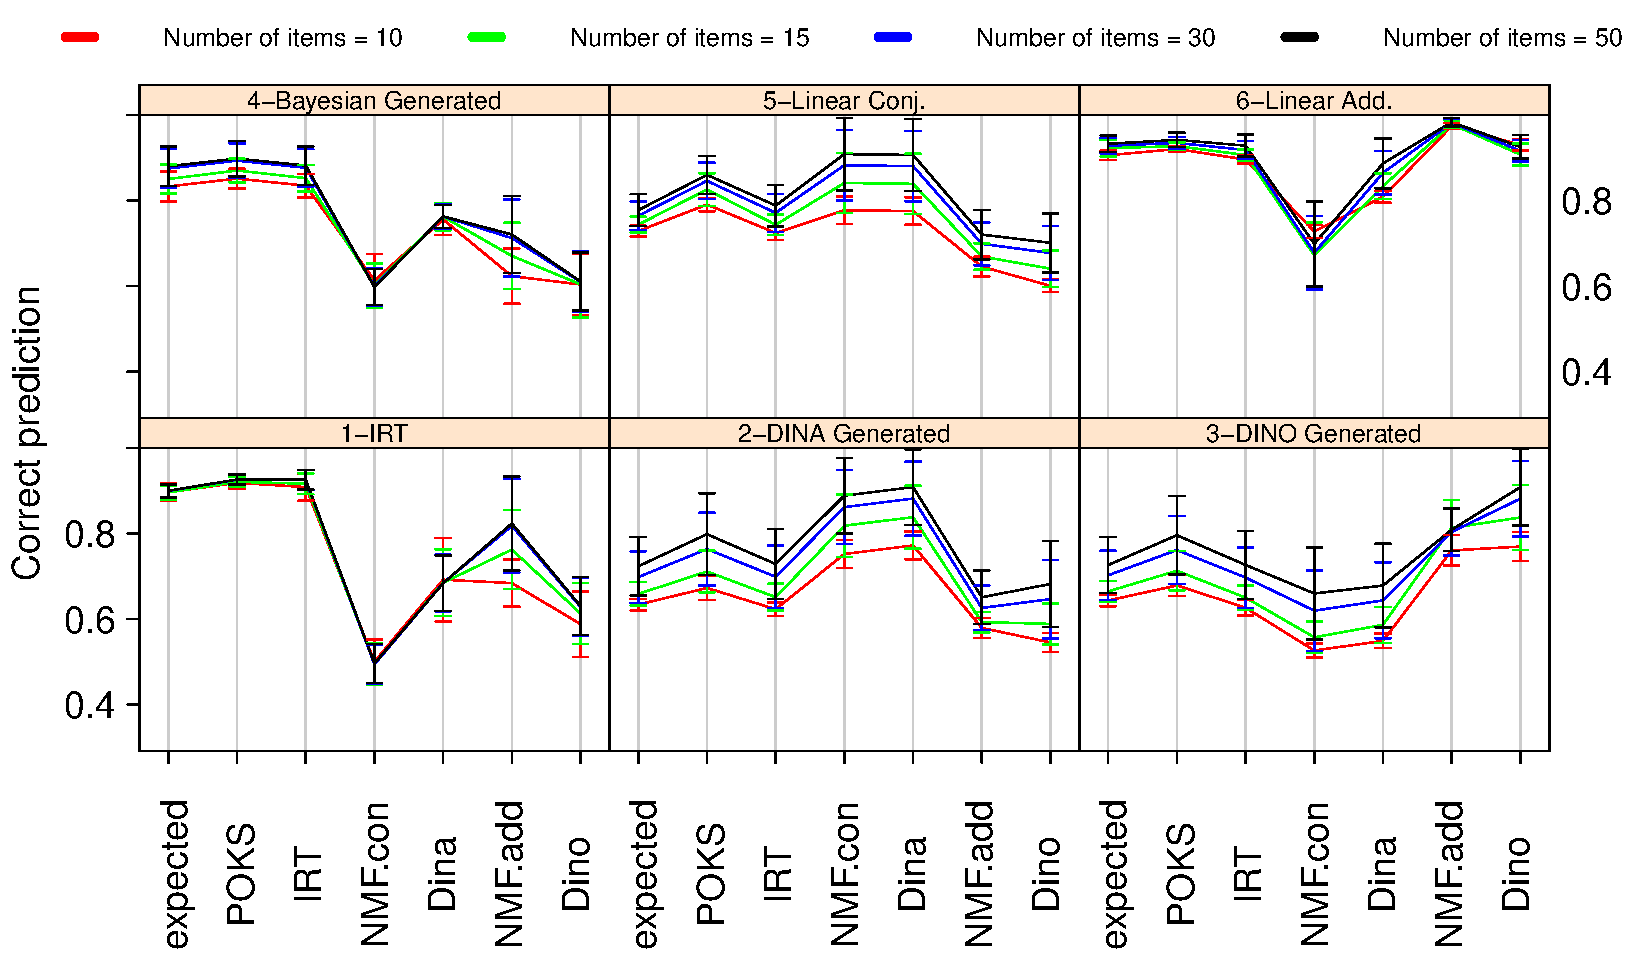
\includegraphics[scale=0.58]{numberofitems.pdf}
\caption{Variation of \textbf{Number of items} Over synthetic data sets}
\label{figNumberofItems}
\end{figure}

\begin{figure}
  \centering
    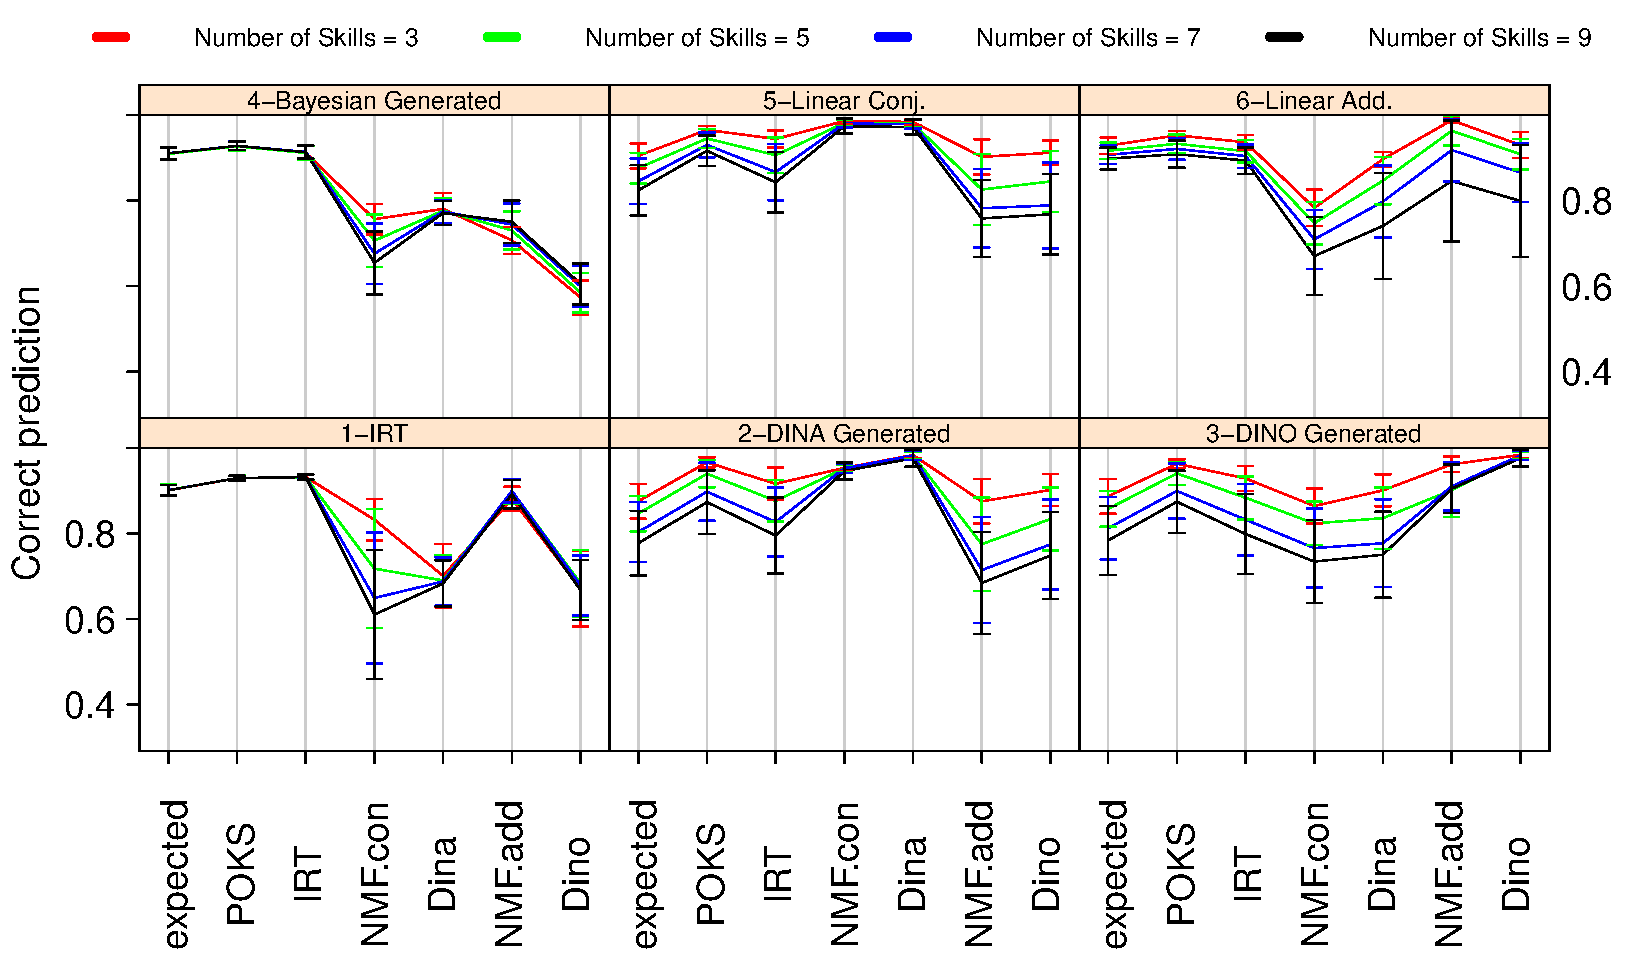
\includegraphics[scale=0.58]{numberofskills.pdf}
\caption{Variation of \textbf{Number of skills} Over synthetic data sets}
\label{figSkills}
\end{figure}

Next variable is number of skills in generation of dataset and estimation of the signature. Same as before we fixed all the other variables to generate the dataset but the number of skills behind the generation of the synthetic dataset which has been in the range of 3 to 9 skills in total. Figure~\ref{figSkills} shows the result of this experiment. For IRT and POKS generated dataset it does not make sense to have number of skills because IRT is a single skill model and there are no explicit latent skills. In order to find the predictive performance of linear methods for bayesian or IRT generated datasets we need to have a fixed number of skills as a part of prediction and that is how we run the experiment with different number of latent skills. The signature pattern did not change substantially for these datasets. Only for linear based techniques we can find a slight change in the pattern. For linear models the pattern still stays the same but for NMF additive when the number of skills increases the ground truth is not the highest performance in the signature. Increasing the number of skills while the number of item is constant can resemble the single skill modeling such as IRT and POKS. 

Figure~\ref{figitemVar} shows the same experiment across datasets with different item variance. The item variance was reflected as the item difficulty for IRT and initial odds for POKS. The value for item variance shows the standard divination of the normal distribution of the items. Clearly the pattern stays the same for different values except for few minor changes. Although the the set of performance values shifts across correct prediction axis but the pattern stays the same.

Finally, we did a last experiment on datasets with different success rates. For synthetic data, the success rate starts from 0.25\% up to 0.85\%. The pattern is scaled for some linear methods on IRT and bayesian generated data and it doesn't change the performance of IRT and POKS themselves. For datasets with linear structure the signature was shifted downward on linear methods predictive performance side as we decrease the success rate for data generation.


\begin{figure}
  \centering
    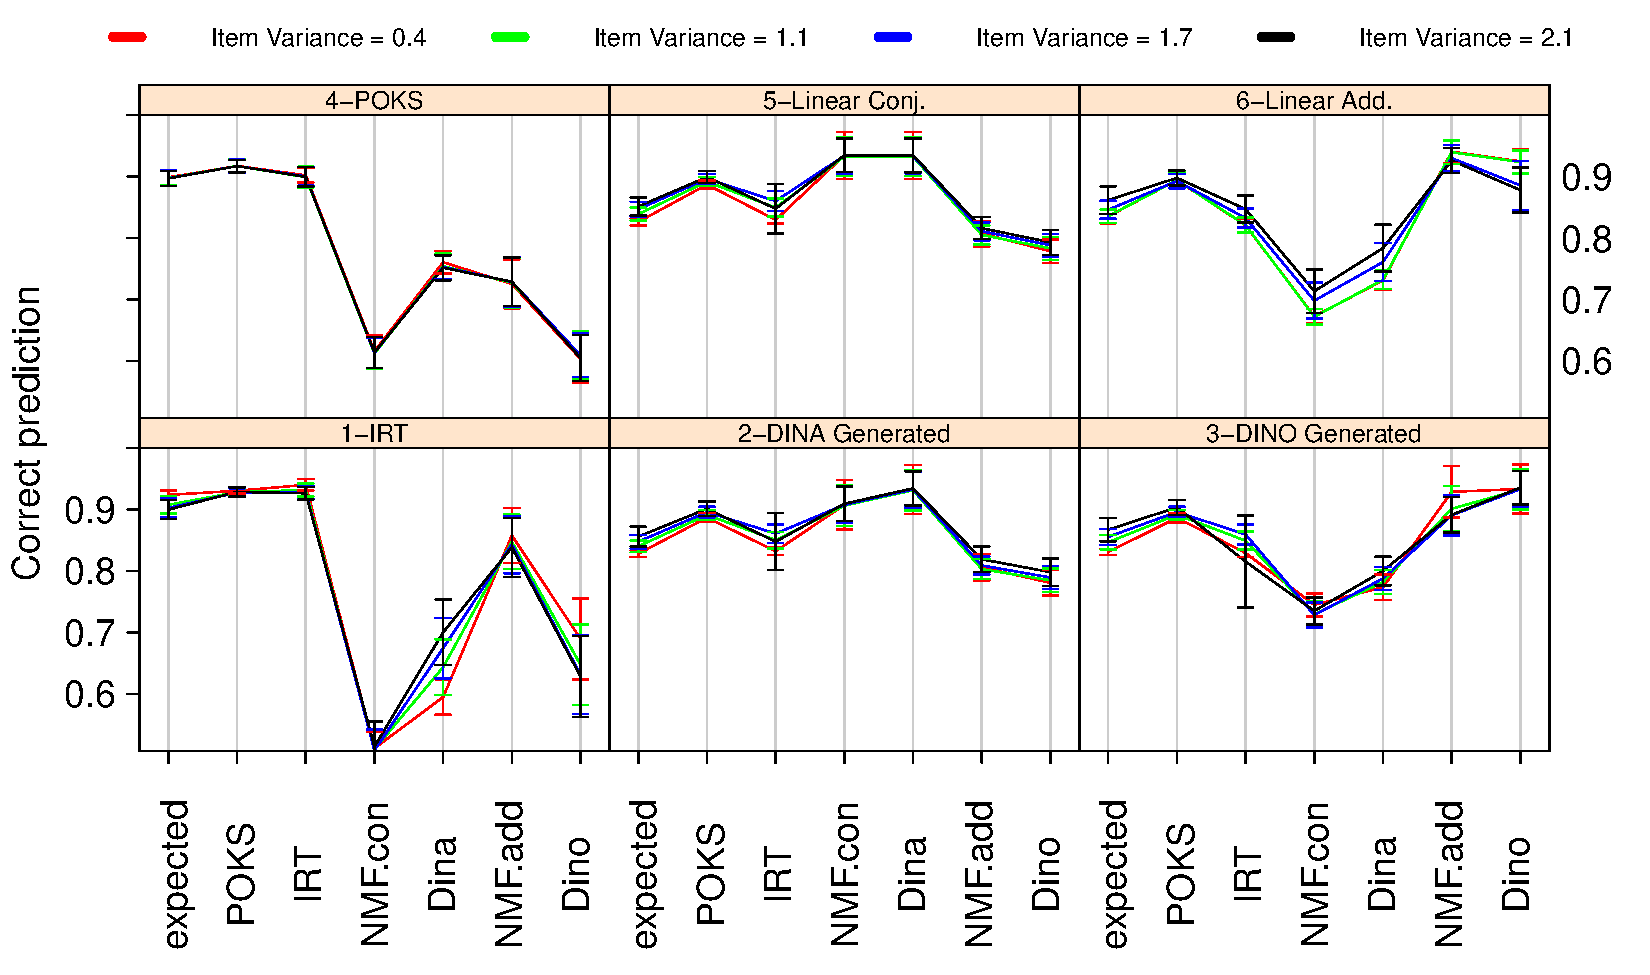
\includegraphics[scale=0.58]{ItemVariance.pdf}
\caption{Variation of \textbf{Item Variance} Over synthetic data sets}
\label{figitemVar}
\end{figure}

\begin{figure}
  \centering
    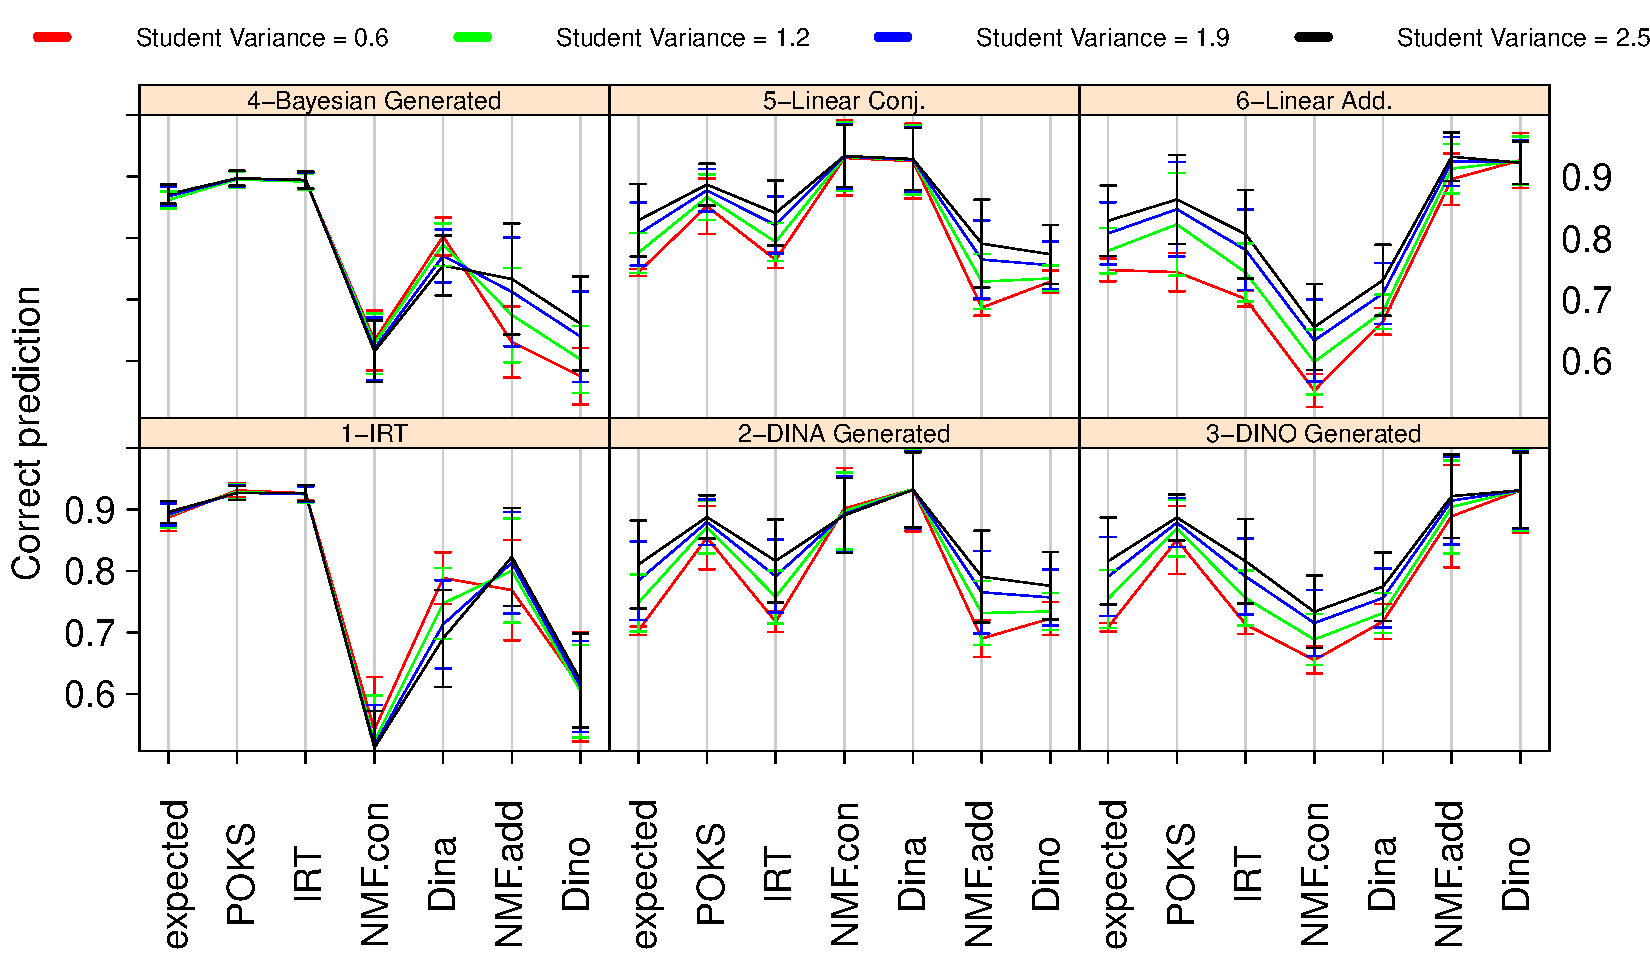
\includegraphics[scale=0.58]{StudentVariance.pdf}
\caption{Variation of \textbf{Student variance} Over synthetic data sets}
\label{figStudentVar}
\end{figure}


\begin{figure}
  \centering
    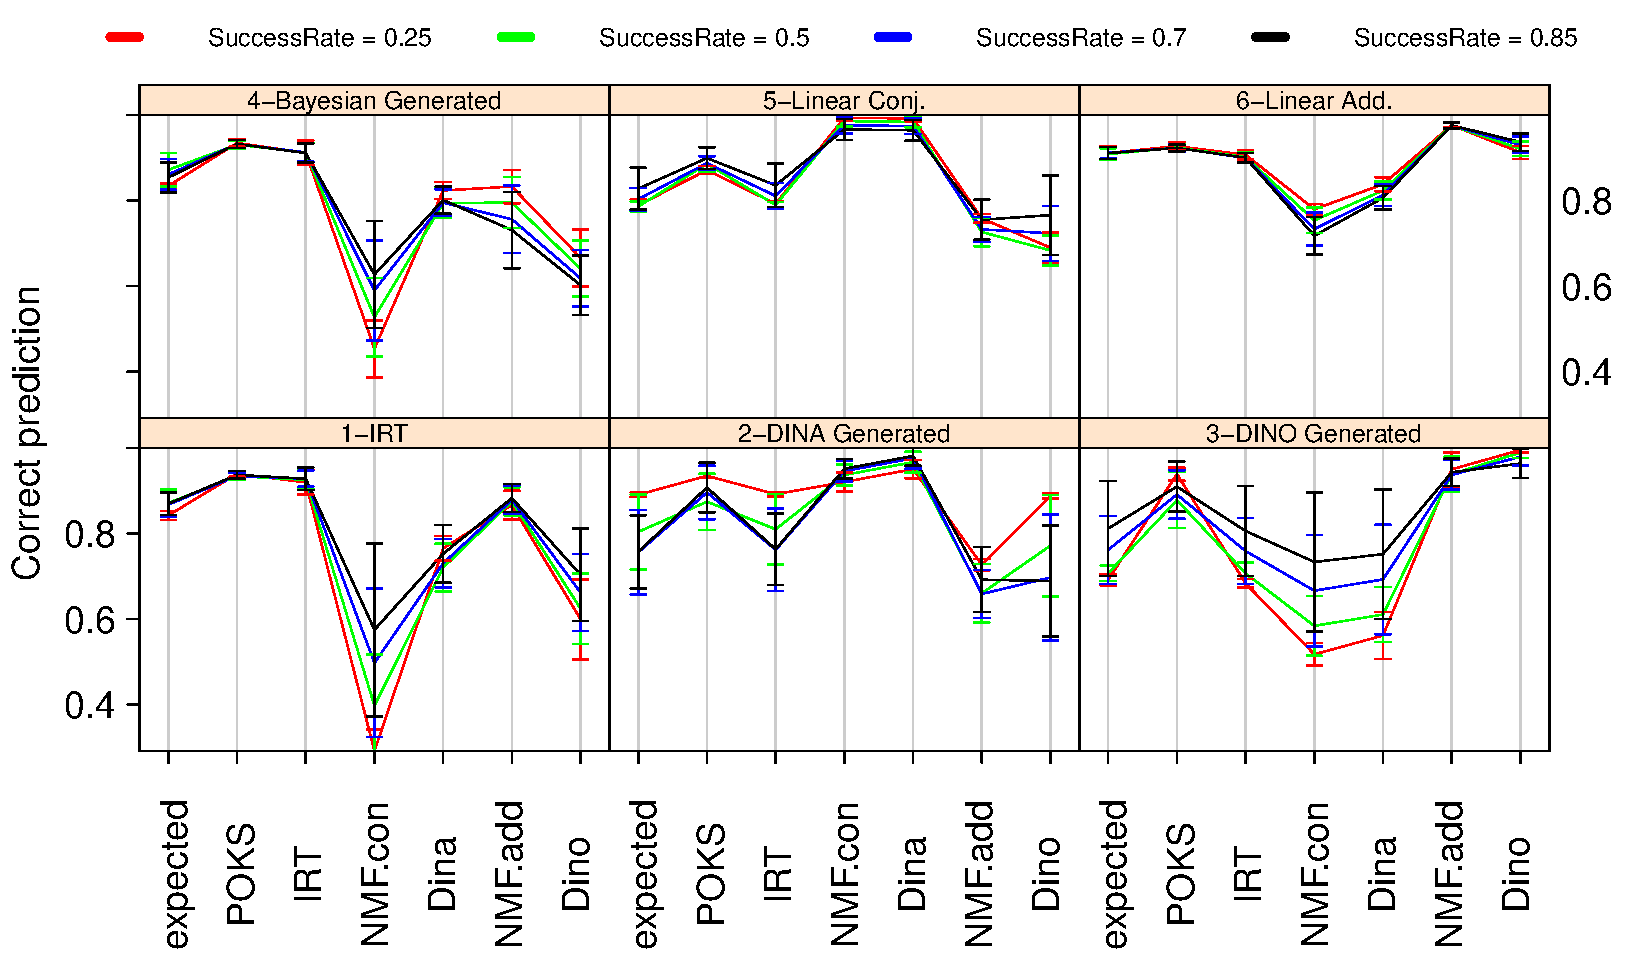
\includegraphics[scale=0.58]{Successrate.pdf}
\caption{Variation of \textbf{Success Rate} Over synthetic data sets}
\label{figSucceessRate}
\end{figure}


\subsection{Degree of similarity}
The most important part is to have a measure to show the degree of similarity between the model performance vector of the synthetic data and the one of the ground truth which is a measure of model fit in our study. Many measures can be used to calculate this degree. The simplest one can be finding the distance between two vector of predictive performance between the synthetic dataset and the real one. previous section showed that different data generation parameters with the same underlying model can create slightly different model performance vectors but with the same pattern. Using distance between each of these signatures with the same ground truth can possibly result in different values for similarity. In this research we used Pearson correlation coefficient as a measure of similarity.


The evaluation of this research consists of two parts. The first part is to measure the degree of similarity for synthetic vs. synthetic datasets. The second part is to identify the ground truth by measuring the correlation between real and synthetic datasets. 

Given $6\times 4$ different set of data generation parameters (described in section \ref{Sensitive}) and generating 10 times for each model will produce 1440 datasets. The comparison in our study is based on same data specific parameters. Therefore we can calculate the correlation table among 60 synthetic datasets that share same data specific parameters. This will result in 24 tables which consider all the possible data generation parameters. The expectation is that those vectors with same model show high correlation. Table \ref{tablSyn} shows the average correlation of these 24  conditions.

Evaluating the synthetic dataset versus themselves can give a clue to how accurate this comparison is in model fitting. Basically, Those datasets that have the same model behind them should show a good correlation. The diagonal of table~\ref{tablSyn} shows a high correlation because it compares the same model generated datasets. On the other hand some models such as IRT and POKS shows a high correlation since they are not using multi-skills models. Those models that share concepts such as DINA and NMF conjunctive also resulted in a high correlation comparing with other models because they are linear models which deal with conjunctive model of Q-matrix. DINO and NMF additive has almost a high correlation but since the additive model is slightly different from the disjunctive model then it's less correlated.


\begin{table}
\center
\begin{tabular}{c|c|c|c|c|c|c|c|}
\multicolumn{2}{c}{} & \multicolumn{6}{c}{Synthetic Datasets} \tabularnewline
\multicolumn{8}{c}{} \tabularnewline
\cline{3-8} 
\multicolumn{2}{c|}{} & POKS & IRT & NMF Conj. & DINA & NMF Add. & DINO\tabularnewline
\cline{2-8}
\cline{2-3}
&POKS & \textbf {0.96} & \multicolumn{1}{|c}{} & \multicolumn{1}{c}{} & \multicolumn{1}{c}{} & \multicolumn{1}{c}{}\tabularnewline
\cline{2-4}
&IRT & 0.86 & \textbf {0.96} & \multicolumn{1}{|c}{} & \multicolumn{1}{c}{} & \multicolumn{1}{c}{} & \multicolumn{1}{c}{}\tabularnewline
\cline{2-5}
&NMF Conj. & 0.22 & -0.20 & \textbf {0.96} & \multicolumn{1}{|c}{} & \multicolumn{1}{c}{} & \multicolumn{1}{c}{}\tabularnewline
\cline{2-6}
&DINA & 0.02 & -0.40 & 0.94 & \textbf {0.96} & \multicolumn{1}{|c}{} & \multicolumn{1}{c}{}\tabularnewline
\cline{2-7}
&NMF Add. & 0.44 & 0.75 & -0.62 & -0.73 & \textbf {0.93} & \multicolumn{1}{|c}{}\tabularnewline
\cline{2-8}
\multicolumn{1}{c|}{\multirow{-6}{*}{\begin{sideways}Synthetic Datasets\end{sideways}}}&DINO & -0.15 & 0.20 & -0.70 & -0.69 & 0.63 & \textbf {0.95}\tabularnewline
\cline{2-8}
\end{tabular}
\caption{Degree of similarity between six synthetic datasets based on the correlation}
\label{tablSyn}
\end{table}



\begin{table}
 \center
\begin{tabular}{c|c|c|c|c|c|c|c|c|}

\multicolumn{2}{c}{}&\multicolumn{7}{c}{Real Datasets}\tabularnewline   
\multicolumn{9}{c}{}\tabularnewline   
\cline{6-9}
\multicolumn{5}{c|}{}&\multicolumn{4}{c|}{Fraction subsets}   \tabularnewline   
\cline{3-9} 
\multicolumn{2}{c|}{}   & Vomlel &ECPE &Fraction &1&21&22&23\tabularnewline
\cline{2-9}
\cline{2-9}
&Random & 0.58 &\textbf {0.73} & 0.61   & 0.43 & 0.24 & 0.61 & 0.57 \tabularnewline
\cline{2-9}
&IRT & \textbf {0.90} & 0.42 & 0.72   & 0.88 & 0.60 & 0.77 & 0.61 \tabularnewline
\cline{2-9}
&DINA & -0.38  & -0.09 &   0.23 &   0.30 & 0.56 & 0.06 & 0.38 \tabularnewline
\cline{2-9}
&DINO & 0.34 & 0.15  &  -0.18 &  -0.31 & 0.10 & -0.08 & 0.38 \tabularnewline
\cline{2-9}
&POKS & 0.75 &0.40  &  \textbf {0.83}  &  \textbf {0.95} &\textbf {0.70} & \textbf {0.83} & \textbf {0.80}\tabularnewline
\cline{2-9}
 &NMF Conj. & -0.05 & 0.54  & 0.51   & 0.55  & 0.66 & 0.33 & 0.57\tabularnewline
\cline{2-9}
\multicolumn{1}{c|}{\multirow{-7}{*}{\begin{sideways}Synthetic Datasets\end{sideways}}}&NMF Add. & 0.39 &0.06   & -0.04   & -0.19 & -0.03 & 0.13 & 0.28\tabularnewline
\cline{2-9}
\end{tabular}
\caption{Degree of similarity between six synthetic datasets and the ground truth based on the correlation}
\label{tablSynReal}
\end{table}


To assess a model fit for each real dataset with this approach we need to create datasets with described underlying models (7 techniques) which have the same parameters of data generation as the real data. Since some parameters influence the performance vector as described in the section~\ref{Sensitive} so we have to create synthetic data that follows the same characteristics of the real one. Table~\ref{tablSynReal} shows the correlation of real data signature in columns with the signature of synthetic data generated with underlying model in rows. Vomlel dataset shows a high correlation with IRT model and Fraction with its subset datasets show similarity with POKS model. As expected ECPE has the highest correlation with random generated dataset.







\begin{table}
\center
\begin{footnotesize}

\begin{adjustwidth}{-0.5cm}{}
\begin{tabular}{c|c!{\VRule[2pt]}c!{\VRule}c!{\VRule[2pt]}c|c!{\VRule[2pt]}c|c!{\VRule[2pt]}c|c!{\VRule[2pt]}c|c!{\VRule[2pt]}c|c!{\VRule[2pt]}c|c|}
\multicolumn{3}{c}{ BP: Best Performer}&\multicolumn{11}{c}{Datasets}&\multicolumn{2}{c}{}\tabularnewline
\cline{15-16}
\multicolumn{3}{c}{ NN: Nearest Neighbor}&\multicolumn{11}{c!{\VRule[2pt]}}{}& \multicolumn{2}{|c|}{Accuracy} \tabularnewline
\cline{3-14}
\multicolumn{2}{c|}{}&\multicolumn{2}{c|}{ POKS}&\multicolumn{2}{c|}{ IRT}&\multicolumn{2}{c|}{ NMF Conj.}&\multicolumn{2}{c|}{ DINA}&\multicolumn{2}{c|}{ NMF Add}&\multicolumn{2}{c!{\VRule[2pt]}}{ DINO}&\multicolumn{2}{c|}{  \scriptsize (\%)}\tabularnewline
\cline{3-16}
\multicolumn{1}{c}{}&\multicolumn{1}{c|}{}&\multicolumn{1}{c|}{ BP}&\multicolumn{1}{c|}{ NN}&\multicolumn{1}{c|}{ BP}&\multicolumn{1}{c|}{ NN}&\multicolumn{1}{c|}{ BP}&\multicolumn{1}{c|}{ NN}&\multicolumn{1}{c|}{ BP}&\multicolumn{1}{c|}{ NN}&\multicolumn{1}{c|}{ BP}&\multicolumn{1}{c|}{ NN}&\multicolumn{1}{c|}{ BP}&\multicolumn{1}{c!{\VRule[2pt]}}{ NN}&\multicolumn{1}{c|}{ BP}&\multicolumn{1}{c|}{ NN}\tabularnewline
\cline{3-16}
\cline{3-16}
\cline{2-16}
\multicolumn{1}{c|}{}& Expected& 0& 0& 0& 0& 0& 0& 0& 0&12& 0& 2& 0& & \tabularnewline
\cline{2-16}
\multicolumn{1}{c|}{}& POKS&\cellcolor{gray!25} 238&\cellcolor{gray!25} 218&130&32&21& 12&14& 0&18&13& 1& 0&85&95\tabularnewline
\cline{2-16}
\multicolumn{1}{c|}{}& IRT& 2& 20&\cellcolor{gray!25}110&\cellcolor{gray!25}208& 0& 0& 0& 0& 0&15& 0& 3&100&97\tabularnewline
\cline{2-16}
\multicolumn{1}{c|}{}& NMF \scriptsize Conj.& 0& 0& 0& 0&\cellcolor{gray!25}82&\cellcolor{gray!25}180& 5&73& 0& 0& 0& 0&100&94\tabularnewline
\cline{2-16}
\multicolumn{1}{c|}{}& DINA& 0& 0& 0& 0&137&48&\cellcolor{gray!25}221&\cellcolor{gray!25}167& 0& 0& 0& 0&87&96\tabularnewline
\cline{2-16}
\multicolumn{1}{c|}{}& NMF \scriptsize Add.& 0& 2& 0& 0& 0& 0& 0& 0&\cellcolor{gray!25}210&\cellcolor{gray!25}211& 14&10&99&99\tabularnewline
\cline{2-16}
\multicolumn{1}{c|}{\multirow{-7}{*}{\begin{sideways}Models\end{sideways}}}& DINO& 0& 0& 0& 0& 0& 0& 0& 0& 0& 1&\cellcolor{gray!25}223&\cellcolor{gray!25}227&100&100\tabularnewline
\cline{1-16}
\multicolumn{2}{|c!{\VRule[2pt]}}{ Accuracy \scriptsize (\%)} & 99 & 91 & 46 & 87 &34 & 75 & 92 & 70 & 88 & 87 & 93 & 95&\multicolumn{2}{|c}{}\tabularnewline
\cline{1-14}
\end{tabular}
\end{adjustwidth}

\end{footnotesize}

\caption{Confusion matrix for classification of 210 synthetic datasets on 7 models with Best performer Vs. Nearest neighbor methods}
\label{Classification-Conf}
\end{table}










\begin{table}
\center	
%\begin{scriptsize}
\begin{tabular}{c|c|c|c|c|c!{\VRule[2pt]}c|c|c|c|}
\multicolumn{2}{c}{}&\multicolumn{8}{c}{Performance}\tabularnewline
\cline{3-10}
\multicolumn{2}{c|}{}&\multicolumn{4}{c|}{Best Performer}&\multicolumn{4}{c|}{Nearest Neighbor}\tabularnewline
\cline{3-10}
\multicolumn{2}{c|}{}&\scriptsize Precision&\scriptsize Recall&\multicolumn{1}{c|}{\scriptsize F-Measure}&\scriptsize Accuracy&\scriptsize Precision&\scriptsize Recall&\scriptsize F-Measure&\scriptsize Accuracy\tabularnewline
\cline{2-10}
&POKS&0.564&0.992&0.719&0.871&0.793&0.908&\cellcolor{gray!25}0.847&\cellcolor{gray!25}0.945\tabularnewline
\cline{2-10}
&IRT&0.982&0.458&0.625&0.908&0.846&0.867&\cellcolor{gray!25}0.856&\cellcolor{gray!25}0.951\tabularnewline
\cline{2-10}
&NMF Conj.&0.943&0.342&0.502&0.887&0.711&0.750&\cellcolor{gray!25}0.730&\cellcolor{gray!25}0.907\tabularnewline
\cline{2-10}
&DINA&0.617&0.921&0.739&0.891&0.777&0.696&\cellcolor{gray!25}0.734&\cellcolor{gray!25}0.916\tabularnewline
\cline{2-10}
&NMF Add.&0.938&0.875&0.905&0.969&0.946&0.879&\cellcolor{gray!25}0.911&\cellcolor{gray!25}0.971\tabularnewline
\cline{2-10}
\multicolumn{1}{c|}{\multirow{-7}{*}{\begin{sideways}Models\end{sideways}}}&DINO&1&0.929&\cellcolor{gray!25}0.963&\cellcolor{gray!25}0.988&0.996&0.946&\cellcolor{gray!25}0.970&\cellcolor{gray!25}0.990\tabularnewline
\cline{2-10}
\end{tabular}
\caption{Accuracy of best performer and nearest neighbor classification methods  }
\label{Classification-Acc}
\end{table}
The very last experiment that we have done is a comparison between the proposed approach where the nearest neighbor classifies in the performance vector space and the simplest approach where the best performer is defining the ground truth. The process is straightforward which is preforming a classification for all synthetic data with best performer method. For the nearest neighbor approach the classification should be done where datasets have the same data generation conditions. Therefore we'll get 24 sets of datasets where similar dara generation parameters exists among each set.Since we have 10 runs for each data specific parameter set then we choose 10 nearest neighbor and preform majority voting on the classification results.

 Table~\ref{Classification-Conf} shows the confusion matrix of this experiment. There exists 1440~datasets where each model corresponds to 240 dataset. The gray cells in table~\ref{Classification-Conf} shows the true positive values and other values in each column represent the false positive predictions for group of datasets.The values in each row shows the number of false negative predictions for each model. The confusion is mostly between those techniques that shares same concepts specially between NMF Conjunctive and DINA model where we use conjunctive Q-matrices. 

The accuracy that is reported in the last row of table~\ref{Classification-Conf} is calculated based on $\frac{TP}{240}$ which counts the true positive predictions for each sub set of datasets that have the same model behind them. The accuracy the is reported in the last two columns of table~\ref{Classification-Conf} is considering how faithful the classification is to select a dataset that doesn't have the related model behind it which will count true negative values based on $\frac{TN}{1200}$ (1200 is the number of datasets that do not have same underlaying models). In terms of true positive selections there is no benefit between any of these methods even sometimes best performer shows to be better (specially for DINA and IRT). 

Considering the false negative and false positive changes the classification results. Table~\ref{Classification-Acc} shows the accuracy of this classification in terms of precision, recall, $F1$ measure and accuracy ($\frac{TN+TP}{1440}$) . Since $F1$ measure is combining both precision and recall, then it is a good measure for improvement. The third column of each classification method shows that F-measure increased for Nearest neighbor method which is almost close to $1$. Also in terms of individual scores per method we also report accuracy of each technique which considers true positive and true negative values. The last column of table~\ref{Classification-Acc} shows this improvement. The total accuracy which is considering true positive numbers over number of datasets regardless of individual models shows that best performer  gets $0.75\%$ and the nearest neighbor gets upto $0.84\%$ of accuracy.


